% !TEX root = ../../main.tex

\section{Schémas numériques}
\label{sec:3:scheme}

\subsection{Méthode de \emph{splitting} hamiltonien}
% -------------------------------------------------------------------

Nous utilisons ici une méthode de \emph{splitting} hamiltonien. Pour le modèle $1dz-3dv$ celui-ci se décompose en 4 étapes, et il s'écrit sous la forme :
\begin{equation}
  \begin{aligned}
    & \partial_t U = \{ U,\mathcal{H}_{j_c}\} + \{ U,\mathcal{H}_B\} + \{ U,\mathcal{H}_E\} + \{ U,\mathcal{H}_{f_h}\} \\
    & U(t=0) = U_0
  \end{aligned}
  \label{eq:hamsplitting}
\end{equation}

Nous allons nous intéresser au calcul de $\varphi_t^{[j_c]}$, $\varphi_t^{[B]}$, $\varphi_t^{[E]}$ et $\varphi_t^{[f_h]}$ les solutions correspondant à chaque étape de sorte que $\varphi(U_0)$ de~\eqref{eq:hamsplitting} peut être approximé au temps $t$ avec une composition des sous-flux $\varphi_t^{[j_c,B,E,f_h]}$.

\paragraph{Étape $\mathcal{H}_{j_c}$ :}
Pour obtenir $\varphi_t^{[j_c]}$, solution du sous-flux $\mathcal{H}_{j_c}$ :
$$
  \begin{cases}
    \partial_t j_{c,\perp} &= -Jj_{c,\perp}B_0 \\
    \partial_t B_\perp     &= 0 \\
    \partial_t E_\perp     &= -j_{c,\perp} \\
    \partial_t f_h         &= 0
  \end{cases}
$$
nous calculons :
$$
  \varphi_t^{[j_c]}(U_0) = \begin{pmatrix}
    e^{-tJ}j_{c,\perp}(0)B_0 \\
    B_\perp(0) \\
    E_\perp(0) - J\left(e^{-tJ}-I\right)j_{c,\perp}(0) \\
    f_h(0)
  \end{pmatrix}
$$
Ce résultat s'obtient grâce à $\int_0^t \exp(-sJ)j_{c,\perp}(0)\,\mathrm{d}s = J\left(\exp(-tJ)-I\right)j_{c,\perp}(0)$.

Nous présentons l'algorithme permettant d'effectuer cette étape dans l'extrait de pseudo-code~\ref{alg:Hjc}. Dans les calculs de complexité que nous nous proposons de faire ici, seuls les parcours de tableaux nous intéressent, la complexité des fonctions mathématiques est supposée constante. Cette étape a une complexité de $\order{N_z}$ en temps.
\begin{algorithm}
  \caption{Calcul de l'étape $\mathcal{H}_{j_c}$}
  \label{alg:Hjc}
  \begin{algorithmic}[1]
    \Function{$\mathcal{H}_{j_c}$}{$j_{c,x}$,$j_{c,y}$,$B_x$,$B_y$,$E_x$,$E_y$,$\hat{f}_h$}
      \For{$i=0,\dots,N_z-1$}
        \State $\bar{j}_{c,x} \gets j_{c,x,[i]}\cos(\Delta t) - j_{c,y,[i]}\sin(\Delta t) $
        \State $\bar{j}_{c,y} \gets j_{c,x,[i]}\sin(\Delta t) + j_{c,y,[i]}\cos(\Delta t) $
        \State $E_{x,[i]}\gets -j_{c,x,[i]}\sin(\Delta t)     + j_{c,y,[i]}(1-\cos(\Delta t))$
        \State $E_{y,[i]}\gets  j_{c,x,[i]}(\cos(\Delta t)-1) - j_{c,y,[i]}\sin(\Delta t)$
        \State $j_{c,x,[i]} \gets \bar{j}_{c,x}$
        \State $j_{c,y,[i]} \gets \bar{j}_{c,y}$
      \EndFor
    \EndFunction
  \end{algorithmic}
\end{algorithm}


\paragraph{Étape $\mathcal{H}_B$ :}
Nous souhaitons calculer $\varphi_t^{[B]}$, correspondant à la solution du système :
$$
  \begin{cases}
    \partial_t j_{c,\perp} &= 0 \\
    \partial_t B_\perp     &= 0 \\
    \partial_t E_\perp     &= -J\partial_zB_\perp \\
    \partial_t f_h         &= 0
  \end{cases}
$$
qui s'obtient de la manière suivante :
$$
  \varphi_t^{[B]}(U_0) = \begin{pmatrix}
    j_{c,\perp}(0) \\
    B_\perp(0) \\
    E_\perp(0) - tJ\partial_zB_\perp(0) \\
    f_h(0)
  \end{pmatrix}
$$
Cette étape est résolu dans l'espace de Fourier, on obtient alors l'algorithme~\ref{alg:HB}. Pour obtenir la complexité de cette étape il faut connaître la complexité de l'algorithme de transformée de Fourier rapide : $\text{FFT}$ que l'on effectue selon l'axe $z$. L'implémentation naïve de cet algorithme est en $\order{N_z^2}$, mais il est possible de descendre à une complexité de $\order{N_z\log(N_z)}$ qui est la valeur que nous considèrerons. La complexité de la transformée de Fourier inverse, $i\text{FFT}$, est la même. On obtient ainsi une complexité temporelle de $\order{6N_z\log(N_z)+N_z}=\order{N_z\log(N_z)}$. Pour la complexité spatiale, il est à noter que cette étape nécessite l'allocation de 4 tableaux temporaires de taille $N_z$ pour le stockage des transformée de Fourier, donc contenant des valeurs complexes (chaque nombre complexe nécessite le stockage de deux réels à virgule flottante).
\begin{algorithm}
  \caption{Calcul de l'étape $\mathcal{H}_{B}$}
  \label{alg:HB}
  \begin{algorithmic}[1]
    \Function{$\mathcal{H}_{B}$}{$j_{c,x}$,$j_{c,y}$,$B_x$,$B_y$,$E_x$,$E_y$,$\hat{f}_h$}
      \State $\hat{B}_x \gets \text{FFT}_z(B_x)$
      \State $\hat{B}_y \gets \text{FFT}_z(B_y)$
      \State $\hat{E}_x \gets \text{FFT}_z(E_x)$
      \State $\hat{E}_y \gets \text{FFT}_z(E_y)$
      \For{$j=0,\dots,N_z-1$}
        \State $\hat{E}_{x,[j]} \gets \hat{E}_{x,[j]} - i\Delta t \kappa_{[j]} \hat{B}_{y,[j]}$
        \State $\hat{E}_{y,[j]} \gets \hat{E}_{y,[j]} + i\Delta t \kappa_{[j]} \hat{B}_{x,[j]}$
      \EndFor
      \State $E_x \gets i\text{FFT}_z(\hat{E}_x)$
      \State $E_y \gets i\text{FFT}_z(\hat{E}_y)$
    \EndFunction
  \end{algorithmic}
\end{algorithm}

\paragraph{Étape $\mathcal{H}_E$ :}
Pour calculer la solution du sous-flux correspondant à $\mathcal{H}_E$, nous devons résoudre le système suivant :
$$
  \begin{cases}
    \partial_t j_{c,\perp} &= \Omega_{pe}^2E_{\perp} \\
    \partial_t B_\perp     &= J\partial_zE_\perp \\
    \partial_t E_\perp     &= (0,0)^\top \\
    \partial_t f_h         &= E_\perp\cdot\nabla_{v_\perp}f_h
  \end{cases}
$$

Avec la condition initiale donnée par $U(t=0)=U_0=(j_{c,\perp},B_\perp,E_\perp,f_h)(t=0)$, la solution au temps $t$ est obtenue par :
$$
  \varphi_t^{[E]}(U_0) = \begin{pmatrix}
    j_{c,\perp} + t\Omega_{pe}^2E_{\perp}(0)\\
    B_\perp(0)+tJ\partial_zE_\perp(0) \\
    E_\perp(0) \\
    f_h(0,z,v_\perp+tE_\perp(0),v_z)
  \end{pmatrix}
$$
Le calcul de $f_h(0,z,v_\perp+tE_\perp(0),v_z)$ s'effectue en utilisant deux interpolations polynomiale de Lagrange d'ordre 5 à une dimension (une dans la direction $v_x$ et une autre dans la direction $v_y$). L'algorithme permettant de résoudre cette étape est présenté dans l'algorithme~\ref{alg:HE}. Les sous-étapes $\mathcal{H}_{E,v_x}$ et $\mathcal{H}_{E,v_y}$ sont très similaires et seul la première est détaillée, seul change l'axe d'interpolation et le pied de la caractéristique. Ces sous-étapes correspondent aux deux interpolations avec un polynôme de Lagrange, faisant appel à la fonction, que l'on ne définit pas ici, $\Call{lagrange\_generator}$ qui permet d'obtenir un polynôme de Lagrange, de degré 5, à partir des 6 points d'interpolations donnés en argument. On considère comme constante la complexité du calcul d'un polynôme d'interpolation, on obtient alors une complexité algorithmique en $\order{N_{v_x}N_{v_y}N_{v_z}N_z}$ pour les sous-étapes $\mathcal{H}_{E,{v_x}}$ et $\mathcal{H}_{E,{v_y}}$. Le calcul de de la transformée de Fourier inverse de $\hat{f}_h$, à la ligne~\ref{alg:HE:l:ifft}, nécessite $N_{v_x}\times N_{v_y}\times N_{v_z}$ transformées de Fourier selon l'axe $z$, soit une complexité totale de $\order{N_{v_x}N_{v_y}N_{v_z}N_z\log(N_z)}$, de même pour la transformée de Fourier à la ligne~\ref{alg:HE:l:fft}. L'étape $\mathcal{H}_{E}$ possède donc une complexité algorithmique de $\order{2N_{v_x}N_{v_y}N_{v_z}N_z + 2N_{v_x}N_{v_y}N_{v_z}N_z\log(N_z) + N_z} = \order{N_{v_x}N_{v_y}N_{v_z}N_z\log(N_z)}$. Pour ce qui concerne l'utilisation de la mémoire, cette étape nécessite deux tableaux de valeurs réelles $f^{(a)}$ et $f^{(b)}$ temporaires de taille $N_{v_x}N_{v_y}N_{v_z}$.
\begin{algorithm}
  \caption{Calcul de l'étape $\mathcal{H}_{E}$}
  \label{alg:HE}
  \begin{algorithmic}[1]
    \Function{$\mathcal{H}_{E,{v_x}}$}{$f^{in}$,$f^{out}$,$E_x$}
      \ForAll{$(k_x,k_y,k_z)\in[\![0,N_{v_x}[\![\times[\![0,N_{v_y}[\![\times[\![0,N_{v_z}[\![$}
        \For{$i=0,\dots,N_z-1$}
          \State $v^{\star} \gets v_x + \Delta t E_{x,[i]}$
          \State $k^{\star} \gets \ceil{\frac{ v^{\star}-v_{x,\text{min}} }{ \Delta v_x }}$
          \State $\mathcal{L}_{[5]} \gets \Call{lagrange\_generator}{f^{in}_{[k^\star-3:k^\star+2,k_y,k_z,i]}}$
          \State $f^{out}_{[k_x,k_y,k_z,i]} \gets \mathcal{L}_{[5]}( v^{\star} )$
        \EndFor
      \EndFor
    \EndFunction
      
      \vspace{0.25cm}

    \Function{$\mathcal{H}_{E}$}{$j_{c,x}$,$j_{c,y}$,$B_x$,$B_y$,$E_x$,$E_y$,$\hat{f}_h$}
      \For{$i=0,\dots,N_z-1$}
        \State $j_{c,x,[i]} \gets j_{c,x,[i]} + \Omega_{pe}^2\Delta t E_{x,[i]}$
        \State $j_{c,y,[i]} \gets j_{c,y,[i]} + \Omega_{pe}^2\Delta t E_{y,[i]}$
      \EndFor
      \State $f^{(a)} \gets i\text{FFT}_z(\hat{f}_h)$ \Comment{La transformée de Fourier inverse s'effectue $\forall v_x,v_y,v_z$}\label{alg:HE:l:ifft}
      \State \Call{$\mathcal{H}_{E,{v_x}}$}{$f^{(a)}$,$f^{(b)}$,$E_x$}
      \State \Call{$\mathcal{H}_{E,{v_y}}$}{$f^{(b)}$,$f^{(a)}$,$E_y$}
      \State $\hat{f}_h \gets \text{FFT}_z(f^{(a)})$ \Comment{La transformée de Fourier s'effectue $\forall v_x,v_y,v_z$} \label{alg:HE:l:fft}
    \EndFunction
  \end{algorithmic}
\end{algorithm}

\paragraph{Étape $\mathcal{H}_{f_h}$ :}
Pour la dernière étape, nous devons calculer une solution du sous-système :
$$
  \begin{cases}
    \partial_t  j_{c,\perp} &= 0 \\
    \partial_t B_\perp      &= 0 \\
    \partial_t E_\perp      &= \int v_\perp f_h\,\mathrm{d}v \\
    \partial_t f_h          &= -v_z\partial_zf_h + (v_yB_0-v_zB_y)\partial_{v_x}f_h + (-v_xB_0+v_zB_x)\partial_{v_y}f_h + (v_xB_y - v_yB_x)\partial_{v_z}f_h
  \end{cases}
$$
Comme pour la résolution de l'équation de Vlasov-Maxwell (\cite{Li:2020}), ce système ne peut être résolu exactement en temps. Mais en suivant \cite{Li:2020}, nous pouvons subdiviser encore l'hamiltonien $\mathcal{H}_{f_h}$ en $\mathcal{H}_{f_h}=\mathcal{H}_{f_{h,x}}+\mathcal{H}_{f_{h,y}}\mathcal{H}_{f_{h,z}}$, où $\mathcal{H}_{f_{h,\star}}=\frac{1}{2}\int v_{\star}^2 f_h\,\mathrm{d}\textbf{v}$, où $\star=x,y,z$. Cela conduit à résoudre les sous-système suivant :

\begin{itemize}
  \item $\mathcal{H}_{f_{h,x}}$ :
    $$
      \begin{cases}
        \partial_t j_{c,\perp} = 0 \\
        \partial_t B_{\perp} = 0 \\
        \partial_t E_{x} = \int v_xf_h\dd{\vb{v}} \\
        \partial_t E_{y} = 0 \\
        \partial_t f_h - (-v_xB_0\partial_{v_y}f_h + v_xB_y\partial_{v_z}f_h) = 0
      \end{cases}
    $$
    On remarque tout d'abord que dans ce sous-système, $\int v_xf_h\dd{\vb{v}}$ est constant en temps, donc l'équation d'Ampère peut être résolue aisément. L'équation de transport sur $f_h$, peut être résolue exactement en utilisant un \emph{splitting} directionnel puisque les deux opérateurs commutent, on obtient alors :
    $$
      \varphi_t^{[f_{h,x}]}(U_0) = \begin{pmatrix}
        j_{c,\perp}(0) \\
        B_{\perp}(0) \\
        E_x(0) + t\int v_xf_h(0)\dd{\vb{v}} \\
        E_y(0) \\
        f_h(0,z,v_x,v_y-tv_xB_0,v_z+tB_yv_x)
      \end{pmatrix}
    $$
    En pratique, nous utiliserons deux interpolations d'ordre 5 avec des polynômes de Lagrange de dimension 1 dans les directions $v_y$ et $v_z$, comme présenté dans l'algorithme~\ref{alg:Hfx}. La sous-étape $\mathcal{H}_{f_{h,x,v_y}}$ n'est qu'une interpolation polynomiale et ne sera pas détaillée ici. La sous-étape $\mathcal{H}_{f_{h,x,v_z}}$ présente en plus la résolution de l'équation d'Ampère, que nous détaillons ici. La complexité de cette étape est $\order{2N_{v_x}N_{v_y}N_{v_z}N_z + N_z} = \order{N_{v_x}N_{v_y}N_{v_z}N_z}$. Pour la complexité spatiale, on remarque la nécessité d'un tableau temporaire de réels $f^{(a)}$ de taille $N_{v_x}N_{v_y}N_{v_z}$.
    \begin{algorithm}
      \caption{Calcul de l'étape $\mathcal{H}_{f_{h,x}}$}
      \label{alg:Hfx}
      \begin{algorithmic}[1]
        \Function{$\mathcal{H}_{f_{h,x,v_z}}$}{$f^{in}$,$f^{out}$,$B_y$,$E_x$}
          \State $j_{h,x} \gets 0$ \Comment{Initialisation d'un tableau de taille $N_z$ à 0}
          \ForAll{$(k_x,k_y,k_z)\in[\![0,N_{v_x}[\![\times[\![0,N_{v_y}[\![\times[\![0,N_{v_z}[\![$}
            \For{$i=0,\dots,N_z-1$}
              \State $v^{\star} \gets v_z + \Delta t v_x B_{y,[i]}$
              \State $k^{\star} \gets \ceil{\frac{ v^{\star}-v_{z,\text{min}} }{ \Delta v_z }}$
              \State $\mathcal{L}_{[5]} \gets \Call{lagrange\_generator}{f^{in}_{[k_x,k_y,k^\star-3:k^\star+2,i]}}$
              \State $f^{out}_{[k_x,k_y,k_z,i]} \gets \mathcal{L}_{[5]}( v^{\star} )$
              \State $j_{h,x,[i]} \gets j_{h,x,[i]} + v_x f^{out}_{[k_x,k_y,k_z,i]} \Delta\vb{v}$
            \EndFor
          \EndFor

          \State $mean \gets \frac{1}{N_z}\sum_i j_{h,x,[i]}$
          \For{$i=0,\dots,N_z-1$}
            \State $E_{x,[i]} \gets E_{x,[i]} + \Delta t(j_{h,x,[i]}-mean)$
          \EndFor
        \EndFunction

          \vspace{0.25cm}

        \Function{$\mathcal{H}_{f_{h,x}}$}{$f^{in}$,$f^{out}$,$B_y$,$E_x$}
          \State \Call{ $\mathcal{H}_{f_{h,x,v_y}}$ }{ $f^{in}$  , $f^{(a)}$ }
          \State \Call{ $\mathcal{H}_{f_{h,x,v_z}}$ }{ $f^{(a)}$ , $f^{out}$ , $B_y$ , $E_x$ }
        \EndFunction
      \end{algorithmic}
    \end{algorithm}

  \item $\mathcal{H}_{f_{h,y}}$ :
    $$
      \begin{cases}
        \partial_t j_{c,\perp} = 0 \\
        \partial_t B_{\perp} = 0 \\
        \partial_t E_{x} = 0 \\
        \partial_t E_{y} = \int v_yf_h\dd{\vb{v}} \\
        \partial_t f_h - (v_yB_0\partial_{v_x}f_h + v_yB_x\partial_{v_z}f_h) = 0
      \end{cases}
    $$
    Cette étape est très similaire à la précédente, le courant des particules chaudes $\int v_yf_h\dd{\vb{v}}$ y est une constante, et l'équation de transport est résolue en utilisant un \emph{splitting} directionnel. On a :
    $$
      \varphi_t^{[f_{h,x}]}(U_0) = \begin{pmatrix}
        j_{c,\perp}(0) \\
        B_{\perp}(0) \\
        E_x(0) \\
        E_y(0) + t\int v_yf_h(0)\dd{\vb{v}} \\
        f_h(0,z,v_x-tv_yB_0,v_y,v_z-tB_xv_y)
      \end{pmatrix}
    $$
    De la même façon, nous utiliserons pour la résolution deux interpolations de dimension 1, interpolation d'ordre 5 à l'aide de polynômes de Lagrange. Nous obtenons les même complexités temporelle et spatiale que l'étape $\mathcal{H}_{f_{h,x}}$.

  \item $\mathcal{H}_{f_{h,z}}$ :
    $$
      \begin{cases}
        \partial_t j_{c,\perp} = 0 \\
        \partial_t B_{\perp} = 0 \\
        \partial_t E_{\perp} = 0 \\
        \partial_t f_h + v_z\partial_{z}f_h - (-v_zB_y\partial_{v_x}f_h + v_zB_x\partial_{v_y}f_h) = 0
      \end{cases}
    $$
    Le calcul de l'étape $\mathcal{H}_{f_{h,z}}$ nécessite plus de travail. Tout d'abord nous introduisons la fonction $g(t,z,\vb{v}) := f(t,z+tv_z,\vb{v})$ qui satisfait :
    \begin{equation}
      \label{eq:ong}
      \partial_t g + B_y(0,z+tv_z)v_z\partial_{v_x}g - v_zB_x(0,z+tv_z)\partial_{v_y}g = 0
    \end{equation}
    Cette équation de transport peut être résolue exactement en temps. Pour cela, dans un premier temps on regarde les caractéristiques de~\eqref{eq:ong} :
    \begin{equation}
      \dot{v}_x(t) = B_y(0,z(0)+tv_z(0))v_z(0)\ ,\qquad \dot{v}_y(t) = -B_x(0,z(0)+tv_z(0))v_z(0),
    \end{equation}
    celles-ci peuvent être résolues exactement. Les variables $z$, $v_z$, $B_x$ et $B_y$ sont constantes en temps dans cette sous-étape, mais le changement de variable introduit une dépendance en temps. Cela peut être résolu en développant le champ magnétique $B_{\perp}$ en série de Fourier dans la direction $z$, ce qui nous donne :
    $$
      B_{\perp}(t,z) = B_\perp(0,z) = \sum_k \hat{B}_\perp(0,k)e^{ikz},
    $$
    on a alors :
    $$
      B_\perp(0,z+tv_z) = \sum_k\hat{B}_\perp(0,k)e^{ik(z+tv_z)}.
    $$
    On obtient alors, en intégrant l'équation~\eqref{eq:ong} en temps :
    $$
      \begin{aligned}
        v_x(t)  &= v_x(0) + v_z(0) \int_0^t \sum_k \hat{B}_{y}(0, k) e^{ik (z(0)+sv_z(0))} \dd{s}  \\
                &= v_x(0) + v_z(0)  \sum_k \hat{B}_{y}(0, k) e^{ik z(0)} \int_0^t e^{ik s v_z(0)} \dd{s} \\
                &= v_x(0) + \sum_k \hat{B}_{y}(0, k) \frac{1}{ik} e^{ik z(0)} (e^{ikt v_z(0)} -1),
      \end{aligned}
    $$
    tandis que pour l'équation sur $v_y$, nous obtenons :
    $$
      \begin{aligned}
        v_y(t) &= v_y(0) - v_z(0) \int_0^t \sum_k \hat{B}_{x}(0, k) e^{ik (z(0) + s v_z(0))}\,\dd{s} \\
               &= v_y(0) - \sum_k \hat{B}_{x} (0, k)\frac{1}{ik}e^{ik z(0)} (e^{ikt v_z(0)} -1).
      \end{aligned}
    $$
    En remontant les caractéristiques, on peut calculer $g(t,z,\vb{v})$ comme :
    $$
      \begin{aligned}
        g(t, z, \vb{v}) = g\left(0, z, v_x - \sum_k \hat{B}_{y}(0, k) \frac{1}{ik} e^{ik z}(e^{ikt v_z} -1), \right.\\
                                \left.v_y +   \sum_k \hat{B}_{x} (0, k)\frac{1}{ik} e^{ik z}(e^{ikt v_z} -1), v_z\right).  
      \end{aligned}
    $$
    Cela nous permet d'obtenir $f_h(t)$ en effectuant le changement de variable inverse :
    $$
      f(t,z,\vb{v}) = g(t,z-tv_z,\vb{v}).
    $$
    Ces différentes étapes permette de construire l'algorithme~\ref{alg:Hfz} permettant la résolution de ce sous-système. Deux sous-étapes $\mathcal{H}_{f_{h,z,v_x}}$ et $\mathcal{H}_{f_{h,z,v_y}}$, effectuent les interpolations polynomiales d'ordre 5, respectivement dans les directions $v_x$ et $v_y$, nous de détaillerons ici que la première. La complexité algorithmique de l'étape correspond à deux fois celle de la sous-étape $\mathcal{H}_{f_{h,z,v_x}}$ (la sous-étape $\mathcal{H}_{f_{h,z,v_y}}$ étant très similaire). Cette étape consiste une transformée de Fourier suivant l'axe $z$ (de complexité $\order{N_z\log(N_z)}$), puis pour toute valeur de $(k_x,k_y,k_z,j)\in[\![0,N_{v_x}[\![\times[\![0,N_{v_y}[\![\times[\![0,N_{v_z}[\![$, une somme sur $N_z$ et une interpolation polynomiale que l'on a supposé de complexité constante. On obtient une complexité algorithmique pour les sous-étapes $\mathcal{H}_{f_{h,z,v_x}}$ et $\mathcal{H}_{f_{h,z,v_y}}$ de $\order{N_z\log(N_z)+N_{v_x}N_{v_y}N_{v_z}N_z^2}$. La sous-étape $\mathcal{H}_{f_{h,z,z}}$, consiste en une transformée de Fourier dans la direction $z$ (de complexité $\order{N_z\log(N_z)}$) et un parcours dans la direction $z$, pour toute valeur d'indices du quadruplet $(k_x,k_y,k_z,j)$, ce qui correspond à une complexité de $\order{N_{v_x}N_{v_y}N_{v_z}(N_z\log(N_z)+N_z)}$. On obtient une complexité algorithmique de l'étape $\mathcal{H}_{f_{h,z}}$ de :
    $$
      \order{2N_z\log(N_z) + N_{v_x}N_{v_y}N_{v_z}N_z(N_z + \log(N_z) + 1)}=\order{N_{v_x}N_{v_y}N_{v_z}N_z^2}.
    $$
    \begin{algorithm}
      \caption{Calcul de l'étape $\mathcal{H}_{f_{h,z}}$}
      \label{alg:Hfz}
      \begin{algorithmic}[1]
        \Function{ $\mathcal{H}_{f_{h,z,v_x}}$ }{ $f^{in}$ , $f^{out}$ , $B_y$ }
          \State $\hat{B}_y \gets \text{FFT}_z(B_y)$
          \ForAll{$(k_x,k_y,k_z)\in[\![0,N_{v_x}[\![\times[\![0,N_{v_y}[\![\times[\![0,N_{v_z}[\![$}
            \For{$j=0,\dots,N_z-1$}
              \State $s \gets -\sum_{\ell=-N_z/2}^{N_z/2} i\frac{\hat{B}_{y,[\ell]}}{\kappa_{[\ell]}}\exp(i\kappa_{[\ell]}z_{[j]})(\exp(i\kappa_{[\ell]}v_z\Delta t) - 1)$

              \State $v^{\star} \gets v_x - \Re(s)$
              \State $k^{\star} \gets \ceil{\frac{ v^{\star}-v_{x,\text{min}} }{ \Delta v_x }}$
              \State $\mathcal{L}_{[5]} \gets \Call{lagrange\_generator}{f^{in}_{[k^\star-3:k^\star+2,k_y,k_z,j]}}$
              \State $f^{out}_{[k_x,k_y,k_z,j]} \gets \mathcal{L}_{[5]}( v^{\star} )$
            \EndFor
          \EndFor
        \EndFunction

          \vspace{0.25cm}

        \Function{ $\mathcal{H}_{f_{h,z,z}}$   }{ $f^{in}$ , $\hat{f}^{out}$ }
          \ForAll{$(k_x,k_y,k_z)\in[\![0,N_{v_x}[\![\times[\![0,N_{v_y}[\![\times[\![0,N_{v_z}[\![$}
            \State $\hat{f}_{\vb{v}} \gets \text{FFT}_z(f^{in}_{[k_x,k_y,k_z,\cdot]})$
            \For{$j=0,\dots,N_z-1$}
              \State $\hat{f}^{out}_{[k_x,k_y,k_z,j]} \gets \hat{f}_{\vb{v},[j]}\exp(-iv_x\kappa_{[j]}\Delta t)$
            \EndFor
          \EndFor
        \EndFunction

          \vspace{0.25cm}

        \Function{ $\mathcal{H}_{f_{h,z}}$ }{ $f^{in}$ , $B_x$ , $B_y$ , $\hat{f}^{out}$ }
          \State \Call{ $\mathcal{H}_{f_{h,z,v_x}}$ }{ $f^{in}$  , $f^{(a)}$       , $B_y$ }
          \State \Call{ $\mathcal{H}_{f_{h,z,v_y}}$ }{ $f^{(a)}$ , $f^{(b)}$       , $B_x$ }
          \State \Call{ $\mathcal{H}_{f_{h,z,z}}$   }{ $f^{(b)}$ , $\hat{f}^{out}$ }
        \EndFunction
      \end{algorithmic}
    \end{algorithm}
\end{itemize}

Finalement, la solution de $\mathcal{H}_{f_h}$ est calculée dans l'algorithme~\ref{alg:Hfh}, qui est une simple composition des sous-étapes $\mathcal{H}_{f_{h,x}}$, $\mathcal{H}_{f_{h,y}}$ et $\mathcal{H}_{f_{h,z}}$. La complexité algorithmique est donc la somme des complexités de chaque sous-étape, ce qui revient, de manière asymptotique, à la complexité de la sous-partie la plus coûteuse, c'est-à-dire $\mathcal{H}_{f_{h,z}}$. La complexité algorithmique de $\mathcal{H}_{f_h}$ est $\order{N_{v_x}N_{v_y}N_{v_z}N_z^2}$. On note cependant la nécessité d'avoir des au moins 2 tableaux temporaires $f^{(a)}$ et $f^{(b)}$ de taille $N_{v_x}N_{v_y}N_{v_z}$ de réels, la variable $f^{(c)}$ peut être remplacée par $f^{(a)}$. Cette étape est la plus coûteuse en temps de calcul, elle sera donc placer au milieu de la méthode \emph{splitting} pour former la méthode de Strang.

\begin{algorithm}
  \caption{Calcul de l'étape $\mathcal{H}_{f_h}$}
  \label{alg:Hfh}
  \begin{algorithmic}[1]
    \Function{$\mathcal{H}_{f_h}$}{$j_{c,x}$,$j_{c,y}$,$B_x$,$B_y$,$E_x$,$E_y$,$\hat{f}_h$}
      \State $f^{(a)} \gets i\text{FFT}_z(\hat{f})$
      \State \Call{ $\mathcal{H}_{f_{h,x}}$ }{ $f^{(a)}$ , $f^{(b)}$   , $B_y$ , $E_x$ }
      \State \Call{ $\mathcal{H}_{f_{h,y}}$ }{ $f^{(b)}$ , $f^{(c)}$   , $B_x$ , $E_y$ }
      \State \Call{ $\mathcal{H}_{f_{h,z}}$ }{ $f^{(c)}$ , $\hat{f}_h$ , $B_x$ , $B_y$ }
    \EndFunction
  \end{algorithmic}
\end{algorithm}

Il est par la suite nécessaire de concaténer les étapes $\mathcal{H}_{j_c}$, $\mathcal{H}_{B}$, $\mathcal{H}_{E}$ et $\mathcal{H}_{f_h}$ pour construire une méthode de Lie, de Strang ou de Suzuki (voir section~\ref{ssec:2:suzuki} ou~\cite{Suzuki:1990} et~\cite{Blanes:2019}). Il est à noter que la méthode Lie possède déjà 4 étapes (11 sous-étapes) et la méthode de Strang 7 (avec 15 sous-étapes, les sous-étapes de $\mathcal{H}_{f_h}$ n'ayant pas besoin d'être concaténées en palindrome). Pour des raisons de temps de calcul, la méthode de Suzuki, avec 35 étapes (soit 75 sous-étapes) ne sera pas considérée comme alternative valable aux méthodes de Lawson d'ordre élevé.


%%%%%%%%%%%%%%%%%%%%%%%%%%%%%%%%%%%%%%%%%%%%%%%%%%%%%%%%%%%%%%%%%%%%%

\FloatBarrier
\subsection{Méthode de Lawson sur le modèle hybride}
% -------------------------------------------------------------------

Dans cette section nous allons présenter la méthode d'intégration exponentielle pour discrétiser le modèle VHL~\eqref{eq:VHM:jx}-\eqref{eq:VHM:fh}. Il est naturel de réécrire ce système, après une transformée de Fourier dans la direction $z$, sous la forme :
$$
  \partial_t U = LU + N(t,U)
$$
où $\kappa=\frac{2j\pi}{N_z}$, $j\in[\![-\frac{N_z}{2},\frac{N_z}{2}]\!]$ représente les modes de Fourier et avec :
\begin{equation}
  L = \begin{pmatrix}
    0   & -B_0 & 0          &  0          &  \Omega_{pe}^2 & 0             & 0 \\
    B_0 &  0   & 0          &  0          &  0             & \Omega_{pe}^2 & 0 \\
    0   &  0   & 0          &  0          &  0             & i\kappa       & 0 \\
    0   &  0   & 0          &  0          & -i\kappa       & 0             & 0 \\
   -1   &  0   & 0          & -i\kappa    &  0             & 0             & 0 \\
    0   & -1   & i\kappa    &  0          &  0             & 0             & 0 \\
    0   &  0   & 0          &  0          &  0             & 0             & -v_z\partial_z \\
  \end{pmatrix},
  \quad
  N:t,U\mapsto \begin{pmatrix}
    0 \\
    0 \\
    0 \\
    0 \\
    \int v_x f \,\mathrm{d}v \\
    \int v_y f \,\mathrm{d}v \\
    E_{\perp}\cdot\nabla_{v_\perp} f - v\times B\nabla_v f
  \end{pmatrix}
  \label{eq:3:LNmaxwell}
\end{equation}
Mais le calcul de la partie linéaire $e^{\tau L}$ nécessaire pour l'écriture du schéma de la méthode LRK n'est pas réalisable avec \sympy{} ou un autre logiciel de calcul formel. Cela vient de l'expression des valeurs propres, dépendant du temps ($\tau$) et de la discrétisation dans l'espace de Fourier des dérivées spatiales ($\kappa\in\left\{\frac{2\pi j}{L},j\in[\![-N_z,N_z]\!]\right\}$). Pour résoudre ce problème, il est décidé dans un premier temps d'intégrer la partie provenant des équations de Maxwell de $L$ dans la partie non-linéaire $N$. Ce qui nous mène à redéfinir $L$ et $N$ comme :
\begin{equation}
  L = \begin{pmatrix}
    0   & -B_0 & 0 &  0 &  \Omega_{pe}^2 & 0             & 0 \\
    B_0 &  0   & 0 &  0 &  0             & \Omega_{pe}^2 & 0 \\
    0   &  0   & 0 &  0 &  0             & 0             & 0 \\
    0   &  0   & 0 &  0 &  0             & 0             & 0 \\
   -1   &  0   & 0 &  0 &  0             & 0             & 0 \\
    0   & -1   & 0 &  0 &  0             & 0             & 0 \\
    0   &  0   & 0 &  0 &  0             & 0             & -v_z\partial_z \\
  \end{pmatrix},
  \ 
  N:t,U\mapsto \begin{pmatrix}
    0 \\
    0 \\
     i\kappa E_y \\
    -i\kappa E_x \\
    -i\kappa B_y + \int v_x f \,\mathrm{d}v \\
     i\kappa B_x + \int v_y f \,\mathrm{d}v \\
    E_{\perp}\cdot\nabla_{v_\perp} f - v\times B\nabla_v f
  \end{pmatrix}
  \label{eq:3:LNsmaxwell}
\end{equation}
Un logiciel de calcul formel, comme \sympy, permet d'obtenir $e^{\tau L}$ pour toute valeur $\tau\in\mathbb{R}$ :
\begin{equation}
\resizebox{.9\hsize}{!}{$
  e^{\tau L} \approx \begin{pmatrix}
  		 \alpha\cos(\theta^-)+\beta\cos(\theta^+) & \alpha\sin(\theta^-)-\beta\sin(\theta^+) & 0 & 0 & \gamma\sin(\theta^-) + \gamma\sin(\theta^+) & -\gamma\cos(\theta^-) + \gamma\cos(\theta^+) & 0 \\
  		-\alpha\sin(\theta^-)+\beta\sin(\theta^+) & \alpha\cos(\theta^-)+\beta\cos(\theta^+) & 0 & 0 & \gamma\cos(\theta^-) - \gamma\cos(\theta^+) &  \gamma\sin(\theta^-) + \gamma\sin(\theta^+) & 0 \\
    0 & 0 & 1 & 0 & 0 & 0 & 0 \\
    0 & 0 & 0 & 1 & 0 & 0 & 0 \\
    -\delta\sin(\theta^-)-\delta\sin(\theta^+) &  \delta\cos(\theta^-)-\delta\cos(\theta^+) & 0 & 0 &  \beta\cos(\theta^-)+\alpha\cos(\theta^+) & \beta\sin(\theta^-)-\alpha\sin(\theta^+) & 0 \\
    -\delta\cos(\theta^-)+\delta\cos(\theta^+) & -\delta\sin(\theta^-)-\delta\sin(\theta^+) & 0 & 0 & -\beta\sin(\theta^-)+\alpha\sin(\theta^+) & \beta\cos(\theta^-)+\alpha\cos(\theta^+) & 0 \\
    0 & 0 & 0 & 0 & 0 & 0 & e^{-ikv_z\tau} \\
    \end{pmatrix}
$}
\end{equation}
avec $\alpha = 0.378732187481834$, $\beta = 0.621267812518167$, $\gamma = 0.970142500145332$, $\delta = 0.242535625036333$, et $\theta^\pm = \frac{\sqrt{2}}{2}\tau\sqrt{9\pm\sqrt{17}}$.

C'est donc à partir de la matrice $L$ sans les termes provenant des équations de Maxwell, et avec le terme non-linéaire $N$, contenant les termes des équations de Maxwell, définis dans~\eqref{eq:3:LNsmaxwell}, que nous allons construire notre premier schéma de Lawson. Il est important d'avoir une formulation explicite de l'exponentielle de la partie linéaire pour construire un schéma en temps efficace. En effet le calcul numérique de l'exponentielle d'une matrice pour une valeur de $\tau$ et de $k$ données est élevé et ne peut être effectuer en amont de la simulation. Le calcul en amont de ces quantités impose une discrétisation en espace donnée, et empêche la mise en place de méthodes à pas de temps adaptatif. Nous verrons par la suite, dans la section~\ref{s3:approx}, une méthode permettant d'intégrer les termes des équations de Maxwell dans la partie linéaire de la méthode de Lawson.

\subsubsection{Filtrage de l'équation de Vlasov}
% ~~~~~~~~~~~~~~~~~~~~~~~~~~~~~~~~~~~~~~~~~~~~~~~~~~~~~~~~~~~~~~~~~~~

L'équation de Vlasov contient le terme $(\vb{v}\times\vb{B}_0)$ qui introduit une condition de CFL restrictive qui peut être outrepassé en utilisant le changement de variable $w=e^{tB_0J}v$, avec $w=(w_x,w_y)^\top$ et $v=(v_x,v_y)^\top$, pour filtrer ce terme en influençant le moins possible le reste du système. Nous introduisons $g(t,z,w,v_z) = f_h(t,z,\exp(-tB_0J)w,v_z)$ avec :
$$
  e^{-tB_0J} = \begin{pmatrix}
    \cos(tB_0) & -\sin(tB_0) \\
    \sin(tB_0) &  \cos(tB_0)
  \end{pmatrix},
  \quad
  J = \begin{pmatrix}
    0  & 1 \\
    -1 & 0
  \end{pmatrix}
$$
alors on a $\exp(-tB_0J)w = \left( \cos(tB_0)w_x - \sin(tB_0)w_y , \sin(tB_0)w_x + \cos(tB_0)w_y \right)^\top$. On peut désormais dériver l'équation sur $g$ :
\begin{equation}
  \partial_t g + v_z\partial_z g - e^{-tB_0J}\vb{E}\cdot\nabla_w g - \mathcal{T}_{\vb{v}}^{[B_0]}g = 0,
\end{equation}
où $\mathcal{T}_{\vb{v}}^{[B_0]}g$ est donné par :
\begin{equation}
  \begin{aligned}
    \mathcal{T}_{\vb{v}}^{[B_0]}g &:= (\vb{v}\times\vb{B})\cdot_{\vb{v}}f_h \\
                                  & = \begin{pmatrix}
                                    \cos(tB_0)w_x - \sin(tB_0)w_y \\
                                    \sin(tB_0)w_x + \cos(tB_0)w_y \\
                                    v_z
                                  \end{pmatrix}
                                  \times
                                  \begin{pmatrix}
                                     B_x \\ B_y \\ 0
                                  \end{pmatrix} 
                                  \cdot
                                  \begin{pmatrix}
                                    e^{-tB_0J}\nabla_w g \\
                                    \partial_{v_z}g
                                  \end{pmatrix} \\
                                  & = \begin{pmatrix}
                                    v_z(-\cos(tB_0)B_y + \sin(tB_0)B_x) \\
                                    v_z(\sin(tB_0)B_y + \cos(tB_0)B_x) \\
                                    (\cos(tB_0)w_x-\sin(tB_0)w_y)B_y - (\sin(tB_0)w_x+\cos(tB_0)w_y)B_x
                                  \end{pmatrix}
                                  \cdot
                                  \begin{pmatrix}
                                    \partial_{w_x}g \\
                                    \partial_{w_y}g \\
                                    \partial_{v_z}g
                                  \end{pmatrix}
  \end{aligned}
\end{equation}
Le changement de variable impacte également l'équation d'Ampère~\eqref{eq:VHM:Ex}-\eqref{eq:VHM:Ey}, l'intégrale du courant des particules chaudes devient :
$$
  \int\vb{v}f\dd{\vb{v}} = \int(e^{-tB_0J}w)g\dd{w}\dd{v_z},
$$
les équations d'Ampère peuvent alors se réécrire comme :
\begin{equation}
  \partial_t E_\perp = -J\partial_z B_\perp - j_{c,\perp} + \int (e^{-tB_0J}w)g\dd{w}\dd{v_z}.
\end{equation}
Les autres équations restent inchangées. Les termes impactés sont dans la partie non-linéaire de la méthode de Lawson, il n'y a donc aucune implication sur le calcul de l'exponentielle de la matrice de la partie linéaire.

\subsubsection{Calcul de stabilité avec les équations de Maxwell}
% ~~~~~~~~~~~~~~~~~~~~~~~~~~~~~~~~~~~~~~~~~~~~~~~~~~~~~~~~~~~~~~~~~~~
\label{ssec:3:cflMaxwell}

Dans la méthode de Lawson explicite que nous souhaitons mettre en place, nous proposons de placer les équations de Maxwell, équations linéaires, dans la partie non-linéaire (voir~\eqref{eq:3:LNsmaxwell}), entrainant par conséquent une condition de stabilité. Puisque nous résolvons de manière explicite des équations linéaires, il est possible d'effectuer un calcul de cette condition CFL de stabilité induite par les équations de Maxwell. Les termes non-linéaires de l'équation de Vlasov sur les particules chaudes, imposent également une condition de stabilité, que l'on se propose de se restreindre à la condition suivante :
$$
  \left\|\vb{E}+\vb{v}\times \vb{B}\right\|_{\infty} \Delta t \leq \Delta v,
$$
condition que l'on peut estimer numériquement par une première simulation.

\paragraph{Estimation de la condition de stabilité à partir d'une méthode Runge-Kutta :\\}
Il est possible de faire une première estimation de la condition de stabilité en ne considérant que l'équation :
\begin{equation}\label{eq:3:maxeq}
  \dot{U} = A\cdot U
\end{equation}
avec $U = (B_x,B_y,E_x,E_y)^\top$ le vecteur des seules variables impliquées dans les équations de Maxwell, et $A$ la matrice :
$$
  A = \begin{pmatrix}
    0       &  0       &  0       & i\kappa \\
    0       &  0       & -i\kappa & 0       \\
    0       & -i\kappa &  0       & 0       \\
    i\kappa &  0       &  0       & 0 
  \end{pmatrix}
$$
On souhaite résoudre ce problème avec une méthode de type Runge-Kutta, en effet notre choix de partie linéaire dans la méthode de Lawson pour résoudre le système VMHL nous impose de résoudre les équations de Maxwell via une méthode de type Runge-Kutta. La fonction à intégrer en temps par la méthode Runge-Kutta étant linéaire en $U$, on sait que calculer $U^{n+1}$ par une méthode Runge-Kutta revient à multiplier $U^n$ par la fonction de stabilité de la méthode Runge-Kutta choisie, évaluée en $\Delta tA$. On a donc pour une méthode RK(3,3) :
$$
  U^{n+1} = \left(I + \Delta t A + \frac{\Delta t^2}{2}A^2 + \frac{\Delta t^3}{6}A^3 \right)U^n,
$$
et pour une méthode RK(4,4) :
$$
  U^{n+1} = \left(I + \Delta t A + \frac{\Delta t^2}{2}A^2 + \frac{\Delta t^3}{6}A^3 + \frac{\Delta t^4}{24}A^4 \right)U^n.
$$
On note $p_{(s,n)}$ la fonction de stabilité de la méthode Runge-Kutta à $s$ étages et d'ordre $n$ RK($s$,$n$). On appellera par la suite \emph{matrice d'amplification}, la matrice correspondant à l'évaluation de la fonction de stabilité de la méthode RK($s$,$n$) évaluée en $\Delta t A$. Pour des méthodes de type Runge-Kutta à $s$ étages et d'ordre $n$ explicite on a :
$$
  p_{(s,n)}(\Delta t A) = \sum_{k=0}^n \frac{\Delta t^k}{k!}A^k + \sum_{k=n+1}^s c_k\Delta t^kA^k
$$
Ce qui correspond au développement de l'exponentielle jusqu'à l'ordre $n$, plus des termes supplémentaires si $n\neq s$. Pour estimer la CFL de l'équation~\eqref{eq:3:maxeq}, il faut rechercher les valeurs propres de la matrice d'amplification $p_{(s,n)}(\Delta t A)$ de la méthode choisie. Celles-ci dépendent de $\Delta t$ et de $\kappa$, avec les modes de Fourier $\kappa$ qui dépendent directement de la discrétisation en espace choisie, car $\kappa=\frac{2\pi j}{L}$ avec $j \in[\![-\frac{N_z}{2},\frac{N_z}{2} ]\!]$. Pour trouver la condition de stabilité de cette équation il faut donc trouver le couple $(\Delta t,\kappa)$ permettant de garantir que les valeurs propres de $p_{(s,n)}(\Delta t A)$ soient inférieure à 1.

On rappelle que les valeurs propres de $A$ sont : $i\kappa$ et $-i\kappa$, chacune de multiplicité 2, cela nous permet de déterminer les valeurs propres de $p_{(s,n)}(\Delta t A)$ qui sont :
$$
  \begin{aligned}
    p_{(s,n)}( i\kappa\Delta t) &= \sum_{k=0}^n       i^k\frac{\Delta t^k\kappa^k}{k!} + \sum_{k=n+1}^s       i^kc_k\Delta t^k\kappa^k \\
    p_{(s,n)}(-i\kappa\Delta t) &= \sum_{k=0}^n (-1)^ki^k\frac{\Delta t^k\kappa^k}{k!} + \sum_{k=n+1}^s (-1)^ki^kc_k\Delta t^k\kappa^k
  \end{aligned}
$$
Il s'agit de polynômes en $\Delta t\kappa$ que l'on peut réécrire :
$$
  \begin{aligned}
    p_{(s,n)}( i\kappa\Delta t) &=  \sum_{k=0}^{ \floor{\frac{n}{2}}   }(-1)^k\frac{\Delta t^{2k}\kappa^{2k}}{(2k)!}
                                 + i\sum_{k=0}^{ \floor{\frac{n}{2}}-1 }(-1)^k\frac{\Delta t^{2k+1}\kappa^{2k+1}}{(2k+1)!}\\
                                 &\quad+  \sum_{k=\floor{\frac{n}{2}}+1}^{ \floor{\frac{s}{2}}   } (-1)^k c_{2k}\Delta t^{2k}\kappa^{2k}
                                       + i\sum_{k=\floor{\frac{n}{2}}  }^{ \floor{\frac{s}{2}}-1 } (-1)^k c_{2k+1}\Delta t^{2k+1}\kappa^{2k+1} \\
    p_{(s,n)}(-i\kappa\Delta t) &=  \sum_{k=0}^{ \floor{\frac{n}{2}}   }(-1)^k\frac{\Delta t^{2k}\kappa^{2k}}{(2k)!}
                                 - i\sum_{k=0}^{ \floor{\frac{n}{2}}-1 }(-1)^k\frac{\Delta t^{2k+1}\kappa^{2k+1}}{(2k+1)!}\\
                                 &\quad+  \sum_{k=\floor{\frac{n}{2}}+1}^{ \floor{\frac{s}{2}}   } (-1)^k c_{2k}\Delta t^{2k}\kappa^{2k}
                                       - i\sum_{k=\floor{\frac{n}{2}}  }^{ \floor{\frac{s}{2}}-1 } (-1)^k c_{2k+1}\Delta t^{2k+1}\kappa^{2k+1} \\
  \end{aligned}
$$
où l'on remarque que $p_{(s,n)}(-i\kappa\Delta t) = \widebar{p_{(s,n)}(i\kappa\Delta t)}$, donc $\left|p_{(s,n)}(-i\kappa\Delta t)\right|=\left|p_{(s,n)}(i\kappa\Delta t)\right|$. On peut déterminer la condition de stabilité pourles méthodes RK(3,3) et RK(4,4), c'est-à-dire la valeur de $\Delta t\kappa$ telle que $|p_{(n,n)}(i\kappa\Delta t)|=1$, on obtient ainsi respectivement les valeurs $\frac{\sqrt{3}}{\kappa}$ et $\frac{2\sqrt{2}}{\kappa}$ avec $\kappa = \frac{2j\pi}{L}$, $j\in[\![-\frac{N_z}{2},\frac{N_z}{2}]\!]$.


\paragraph{Estimation de la condition de stabilité à partir d'une méthode de Lawson complète :\\}
Une estimation plus précise de la condition de stabilité dû aux équations de Maxwell peut être calculée en résolvant avec une méthode de Lawson le système :
$$
  \dot{U} = LU + NU
$$
où $U = (j_{c,x},j_{c,y},B_x,B_y,E_x,E_y)^\top$, et $L$ (partie linéaire de la méthode de Lawson) et $N$ (partie considérée comme non-linéaire dans la méthode de Lawson) sont deux matrices données par :
$$  L = \begin{pmatrix}
    0 & -1 & 0 & 0 & 4 & 0 \\
    1 &  0 & 0 & 0 & 0 & 4 \\
    0 &  0 & 0 & 0 & 0 & 0 \\
    0 &  0 & 0 & 0 & 0 & 0 \\
   -1 &  0 & 0 & 0 & 0 & 0 \\
    0 & -1 & 0 & 0 & 0 & 0 \\
  \end{pmatrix},
  \ 
  N = \begin{pmatrix}
    0 & 0 & 0  &  0  &  0  & 0  \\
    0 & 0 & 0  &  0  &  0  & 0  \\
    0 & 0 & 0  &  0  &  0  & ik \\
    0 & 0 & 0  &  0  & -ik & 0  \\
    0 & 0 & 0  & -ik &  0  & 0  \\
    0 & 0 & ik &  0  &  0  & 0  \\
  \end{pmatrix}
$$
On ne s'intéresse ici qu'à la condition de stabilité provenant des équations de Maxwell, dû à l'impossibilité de calculer formellement $e^{\tau L}$ avec les équations de Maxwell. La densité de particules $f_h$ n'est donc pas considérée ici. De plus la condition de stabilité que nous cherchons est celle provenant des équations de Maxwell, donc une condition sur la discrétisation spatiale, la condition de stabilité induite par $f_h$ ne porte que sur la discrétisation en vitesse et ne sera pas étudié ici car le terme est fortement non-linéaire. Les matrices $L$ et $N$ ne commutent pas, donc la fonction de stabilité de la méthode de Lawson ne peut pas être obtenu comme dans le cas scalaire du chapitre~\ref{chap1}. Il est nécessaire pour chaque méthode de calculer sa fonction de stabilité. Nous n'étudierons ici que les méthodes de Lawson induites par la méthode RK(3,3) de Shu-Osher et celle induite par la méthode RK(4,4) dites classique.

Nous allons commencer l'étude par la méthode RK(3,3) définie par :
$$
  \begin{aligned}
    U^{(1)} &= e^{\Delta tL}U^n + \Delta te^{\Delta tL}NU^n \\
    U^{(2)} &= \frac{3}{4}e^{\frac{\Delta t}{2}L}U^n + \frac{1}{4}e^{-\frac{\Delta t}{2}L}U^{(1)} + \frac{\Delta t}{4}e^{-\frac{\Delta t}{2}L}NU^{(1)} \\
    U^{n+1} &= \frac{1}{3}e^{\Delta tL}U^n + \frac{2}{3}e^{\frac{\Delta t}{2}L}U^{(2)} + \frac{2}{3}\Delta te^{\frac{\Delta t}{2}L}NU^{(2)} \\
  \end{aligned}
$$
On peut calculer la fonction de stabilité de la méthode, on obtient alors :
$$
  \begin{aligned}
    U^{n+1} = \Big[ e^{\Delta tL} &+ \Delta t\left(\frac{2}{3}e^{\frac{\Delta t}{2}L}Ne^{\frac{\Delta t}{2}L}+\frac{1}{6}e^{\Delta tL}N + \frac{1}{6}Ne^{\Delta tL}\right) \\
    & + \frac{\Delta t^2}{2}\left(\frac{1}{3}Ne^{\Delta tL}N + \frac{1}{3}e^{\frac{\Delta t}{2}L}Ne^{\frac{\Delta t}{2}L}N + \frac{1}{3} e^{\frac{\Delta t}{2}L}Ne^{-\frac{\Delta t}{2}L}Ne^{\Delta tL} \right) \\
    & + \frac{\Delta t^3}{6}e^{\frac{\Delta t}{2}L}Ne^{-\frac{\Delta t}{2}L}Ne^{\Delta tL}N \Big]U^n
  \end{aligned}
$$
La matrice d'amplification n'est plus un polynôme, nous nous proposons donc de faire une étude numérique. Pour cela on choisit une discrétisation des modes de Fourier $\kappa\in[\![-27,27]\!]$, et pour les pas de temps $\Delta t\in[0,0.125]$. Pour tout couple de cette discrétisation on calcule numériquement les valeurs propres de la matrice d'amplification, qui sont au nombre de 5, sans compter la multiplicité, que l'on tri par valeur absolue. Cela nous permet de représenter graphiquement, sur la figure~\ref{fig:3:vplrk33}, la plus grande valeur propre en chaque point $(\kappa,\Delta t)$ de la discrétisation. On remarque une symétrie, attendue, entre les modes de Fourier positifs et négatifs, et c'est le mode le plus élevé qui va contraindre le plus notre condition de stabilité entre $\kappa$ et $\Delta t$.
\begin{figure}[h]
  \centering
  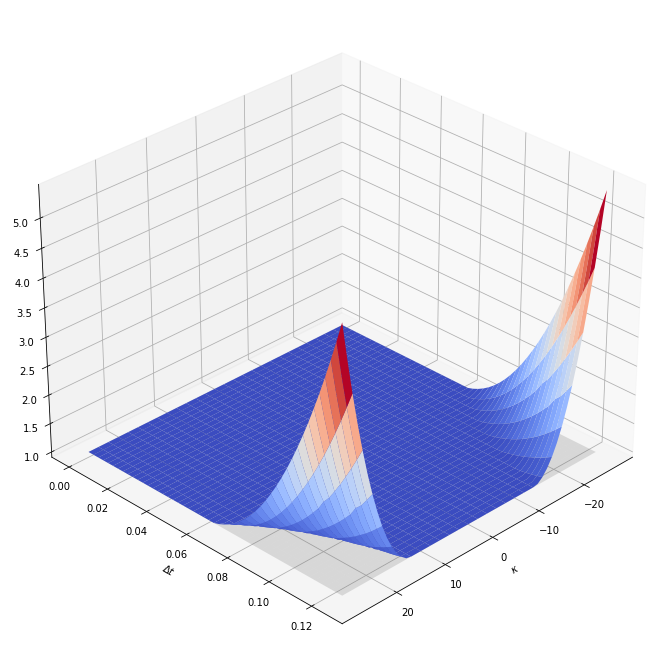
\includegraphics[height=0.49\textheight]{\localPath/figures/vplrk33.png}
  \caption{Plus grande valeur propre en valeur absolue de la matrice d'amplification de la méthode LRK(3,3) sur l'espace discrétisé de $(\kappa,\Delta t)\in[\![-27,27]\!]\times[0,0.125]$}
  \label{fig:3:vplrk33}
\end{figure}
On peut regarder, sur la figure~\ref{fig:3:vpMrk33_k15}, pour le seul mode $\kappa=15$, la valeur absolue des différentes valeurs propres de la matrice d'amplification. On remarque la présence d'une valeur propre égale à 1 ainsi que d'autres valeurs propres, qui sont strictement inférieur à 1 pour des petites valeurs de $\Delta t$ (jusqu'à $0.11$ environ). Pour estimer une condition de stabilité pour $\kappa=15$, il est nécessaire de connaître la valeur de $\Delta t$ telle que la plus grande valeur propre soit de module suppérieur à 1. On trace sur la figure~\ref{fig:3:vpMrk33}, le module de la plus grande valeur propre de la matrice d'amplification, pour différents mode de Fourier $\kappa\in[\![0,27]\!]$. On remarque que plus la discrétisation en $x$ est fine (grande valeur des modes de Fourier) la valeur de $\Delta t$ permettant d'assurer la stabilité diminue.
\begin{figure}[h]
  \centering
  \setbox9=\hbox{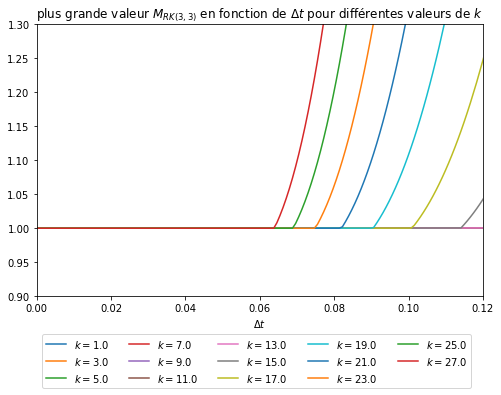
\includegraphics[width=0.45\linewidth]{\localPath/figures/vpMrk33.png}}
  \begin{subfigure}[b]{.45\linewidth}
    \raisebox{\dimexpr\ht9-\height}{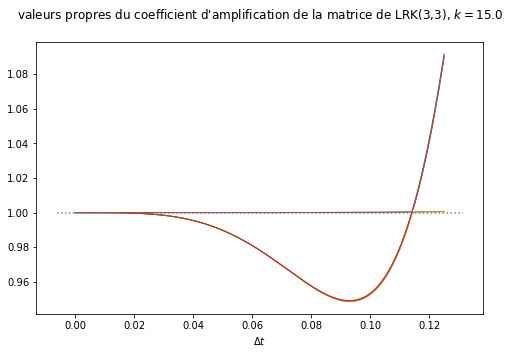
\includegraphics[width=\textwidth]{\localPath/figures/vpMrk33_k15.png}}
    \caption{Module des valeurs propres de la matrice d'amplification de LRK(3,3) pour le mode de Fourier $\kappa=15$, $\Delta t\in[0,0.12]$.\\ }
    \label{fig:3:vpMrk33_k15}
  \end{subfigure}
  \begin{subfigure}[b]{.45\linewidth}
    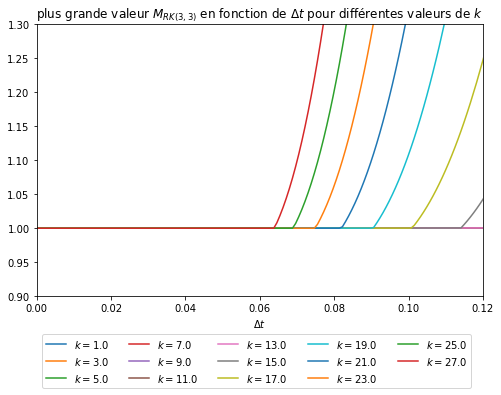
\includegraphics[width=\textwidth]{\localPath/figures/vpMrk33.png}
    \caption{Module de la plus grande valeur propre de la matrice d'amplification de LRK(3,3) pour différents modes de Fourier $\kappa\in[\![0,27]\!]$ et $\Delta t\in[0,0.12]$.}
    \label{fig:3:vpMrk33}
  \end{subfigure}
  \caption{Étude des valeurs propres de la matrice d'amplification de la méthode LRK(3,3) en fonction de $\Delta t$.}
\end{figure}
On peut ainsi estimer une condition de stabilité pour $N_z = 15,27$ et on obtient : pour $N_z = 15$, $\Delta t <0.115 \approx \frac{\sqrt{3}}{15}$, et pour $N_z = 27$, $\Delta t <0.066 \approx \frac{\sqrt{3}}{27}$.

On effectue une analyse similaire pour la méthode de Lawson LRK(4,4) suivante :
$$
  \begin{aligned}
    U^{(1)} &= e^{\frac{\Delta t}{2}L}U^n + \frac{\Delta t}{2}e^{\frac{\Delta t}{2}L}NU^n \\
    U^{(2)} &= e^{\frac{\Delta t}{2}L}U^n + \frac{\Delta t}{2}NU^{(1)} \\
    U^{(3)} &= e^{\Delta tL}U^n + \Delta te^{\frac{\Delta t}{2}L}NU^{(2)} \\
    U^{n+1} &= -\frac{1}{3}e^{\Delta tL}U^n + \frac{1}{3}e^{\frac{\Delta t}{2}L}U^{(1)} + \frac{2}{3}e^{\frac{\Delta t}{2}L}U^{(2)} + \frac{1}{3}U^{(3)} \frac{\Delta t}{6}NU^{(3)} \\
  \end{aligned}
$$
Où l'on peut également calculer sa matrice d'amplification :
$$
  \begin{aligned}
    U^{n+1} = \Big[ e^{\Delta t} 
              & + \Delta t\left( \frac{1}{6}e^{\Delta t L}N + \frac{2}{3}e^{\frac{\Delta t}{2}L}Ne^{\frac{\Delta t}{2}L} + \frac{1}{6}Ne^{\Delta t L} \right) \\
              & + \frac{\Delta t^2}{2} \left( \frac{1}{3}e^{\frac{\Delta t}{2}L}Ne^{\frac{\Delta t}{2}L}N + \frac{1}{3}e^{\frac{\Delta t}{2}L}N^2e^{\frac{\Delta t}{2}L} + \frac{1}{3}Ne^{\frac{\Delta t}{2}L}Ne^{\frac{\Delta t}{2}L} \right) \\
              & + \frac{\Delta t^3}{6} \left( \frac{1}{2}e^{\frac{\Delta t}{2}L}N^2e^{\frac{\Delta t}{2}L}N + \frac{1}{2}Ne^{\frac{\Delta t}{2}L}N^2e^{\frac{\Delta t}{2}L} \right) \\
              & + \frac{\Delta t^4}{24}Ne^{\frac{\Delta t}{2}L}N^2e^{\frac{\Delta t}{2}L}N \Big]U^n
  \end{aligned}
$$
Ce qui nous permet, avec la même discrétisation de $\kappa$ et $\Delta t$ de tracer les mêmes diagnostics que précédemment sur la figure~\ref{fig:3:vplrk44}. On représente ainsi à gauche le module des différentes valeurs propres de la matrice d'amplification de la méthode LRK(4,4) pour $\kappa=15$, et à droite on ne s'intéresse qu'à la plus grande valeur propre pour différents modes de Fourier $\kappa\in[\![0,27]\!]$. Cela nous permet d'obtenir les conditions de stabilité pour différentes discrétisation en espace, et par exemple pour $N_z = 15$ on trouve $\Delta t<0.188 \approx \frac{2\sqrt{2}}{15}$ et pour $N_z = 27$ on trouve $\Delta t < 0.104 \approx \frac{2\sqrt{2}}{27}$.
\begin{figure}[h]
  \centering
  \setbox9=\hbox{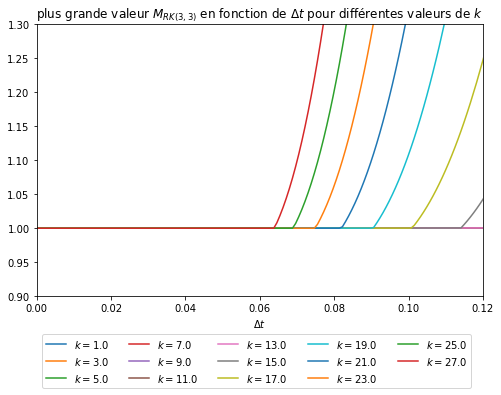
\includegraphics[width=0.45\linewidth]{\localPath/figures/vpMrk33.png}}
  \begin{subfigure}[b]{.45\linewidth}
    \raisebox{\dimexpr\ht9-\height}{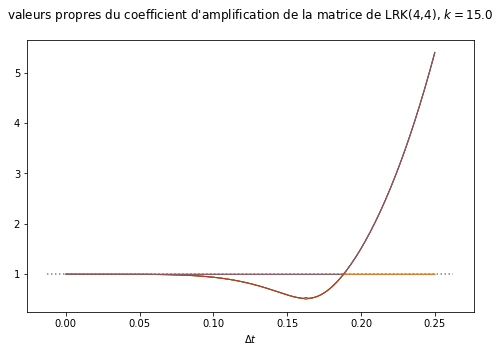
\includegraphics[width=\textwidth]{\localPath/figures/vpMrk44_k15.png}}
    \caption{Module des valeurs propres de la matrice d'amplification de LRK(4,4) pour le mode de Fourier $\kappa=15$, $\Delta t\in[0,0.25]$.\\ }
    \label{fig:3:vpMrk44_k15}
  \end{subfigure}
  \begin{subfigure}[b]{.45\linewidth}
    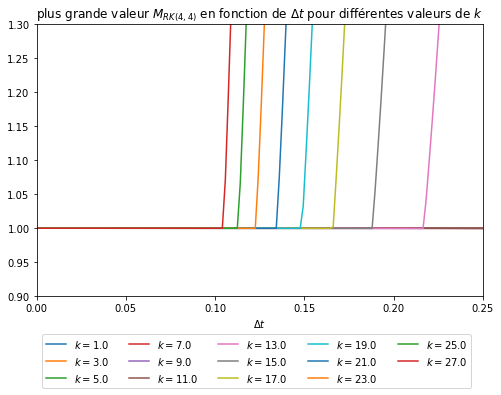
\includegraphics[width=\textwidth]{\localPath/figures/vpMrk44.png}
    \caption{Module de la plus grande valeur propre de la matrice d'amplification de LRK(4,4) pour différents modes de Fourier $\kappa\in[\![0,27]\!]$ et $\Delta t\in[0,0.25]$.}
    \label{fig:3:vpMrk44}
  \end{subfigure}
  \caption{Étude des valeurs propres de la matrice d'amplification de la méthode LRK(4,4) en fonction de $\Delta t$.}
  \label{fig:3:vplrk44}
\end{figure}

Cela conclu l'estimation de condition de stabilité en espace. On remarque que l'estimation numérique de la condition de stabilité de la méthode de Lawson est très proche de la condition de stabilité obtenue à l'aide de la restriction à la résolution de la méthode Runge-Kutta sur $(B_x,B_y,E_x,E_y)^\top$.


\subsubsection{Synthèse d'un étage}
% ~~~~~~~~~~~~~~~~~~~~~~~~~~~~~~~~~~~~~~~~~~~~~~~~~~~~~~~~~~~~~~~~~~~
\label{ssec:3:stage}

Intéressons nous maintenant à l'implémentation de la méthode de Lawson. Les méthodes de type Runge-Kutta s'écrivent comme une succession d'étage et chaque étage possède des expressions différentes mais une structure similaire. Ces premières sont générées à l'aide d'outils de méta-programmation, présentés dans la sous-section~\ref{ssec:3:codegen}, basés sur la bibliothèque \Python{} de calcul symbolique \sympy{}. Le squelette d'un étage est présent dans l'algorithme~\ref{alg:squeltte}. La résolution numérique des dérivées en espace $z$ se font dans l'espace de Fourier, pour cette raison, les variables transmises entres étages ou itérations, sont des tableaux de complexes, correspondant aux modes de Fourier des différentes variables.

L'algorithme d'un étage se comporte en deux grandes sections. La première partie permet de mettre à jour les variables spatiales $(j_{c,x},j_{c,y},B_x,B_y,E_x,E_y)$ dans l'espace de Fourier, qui commence à la ligne~\ref{alg:l:0}, qui commence par le calcul des courants induits par les particules chaudes $\int v_\star f_h\dd{\vb{v}}$ où $\star\in\{x,y\}$ dans l'espace de Fourier. Les lignes~\ref{alg:l:sp0} à~\ref{alg:l:sp5}, sont générées à l'aide d'outils présentés dans la sous-section~\ref{ssec:3:codegen}. La seconde partie permet la mise à jour de $f_h$ dans l'espace de Fourier et commence à la lignes~\ref{alg:l:15}. Cette partie commence par le calcul de $\vb{E}+(\vb{v}\times\vb{B})\cdot\nabla_{\vb{v}}f_h$ à l'aide de la méthode WENO, puis continue par la mise à jour de $f_h$ dans l'espace de Fourier en effectuant la transformée de Fourier en $z$ de $\vb{E}+(\vb{v}\times\vb{B})\cdot\nabla_{\vb{v}}f_h$ pour une vitesse $\vb{v}$ donnée. La ligne~\ref{alg:l:sp6} est également générée automatiquement.

%\Josselin{je ne sais pas si le détail de l'algorithme est très convainquant, je peux aussi ajouter un peu plus de commentaires dans l'algorithme, donc peut-être à voir selon vos retours car j'ai peut-être un peu trop bosser dessus et j'ai un regard moins matheux. Je présume en plus qu'il sera nécessaire d'expliquer les notations où j'ai mis entre crochets les indices dont dépendent les variables, et j'ai utilisé la notation de MATLAB et de \Python{} pour indiquer un ensemble de valeurs entre 2 indices de tableau. Mais je pense que dans la partie \emph{splitting} j'ajouterai aussi des algorithmes pour $\mathcal{H}_{j_c}$, $\mathcal{H}_{B}$, $\mathcal{H}_{E}$, $\mathcal{H}_{f_h}$ donc j'expliquerais les notations à ce moment là.}

\begin{algorithm}
  \caption{Squelette de l'algorithme d'un étage $s$ d'une méthode LRK}
  \label{alg:squeltte}
  \begin{algorithmic}[1]
    \State{$\triangleright$ Calcul des variables $\hat{j}_{c,x}^{(s)}$, $\hat{j}_{c,y}^{(s)}$, $\hat{B}_{x}^{(s)}$, $\hat{B}_{y}^{(s)}$, $\hat{E}_{x}^{(s)}$ et $\hat{E}_{y}^{(s)}$} \label{alg:l:0}

    \For{$i=0,\dots,N_z$}
      \State $\hat{j}_{h,x,[i]} \gets \sum_{k_x,k_y,k_z} v_{k_x}\,\hat{f}_{h,[i,k_x,k_y,k_z]}^{(s-1)}\,\Delta v$ \label{alg:l:jhx}
      \State $\hat{j}_{h,y,[i]} \gets \sum_{k_x,k_y,k_z} v_{k_y}\,\hat{f}_{h,[i,k_x,k_y,k_z]}^{(s-1)}\,\Delta v$ \label{alg:l:jhy}
    \EndFor

    \For{$i=0,\dots,N_z$}
      \State $\hat{j}_{c,x,[i]}^{(s)} \gets \dots$ \Comment{les expressions ici sont données par \sympy}\label{alg:l:sp0}
      \State $\hat{j}_{c,y,[i]}^{(s)} \gets \dots$
      \State $\hat{B}_{x,[i]}^{(s)}   \gets \dots$
      \State $\hat{B}_{y,[i]}^{(s)}   \gets \dots$
      \State $\hat{E}_{x,[i]}^{(s)}   \gets \dots$
      \State $\hat{E}_{y,[i]}^{(s)}   \gets \dots$ \label{alg:l:sp5}
    \EndFor

    \State{$\triangleright$ Calcul de la variable $\hat{f}_h^{(s)}$} \label{alg:l:15}

    \State $\left(f\right)_{h,[\cdot,k_x,k_y,k_z]} \gets \textrm{iFFT}_z\left( \hat{f}^{(s-1)}_{h,[\cdot,k_x,k_y,k_z]} \right)$
    \ForAll{ $(k_x,k_y,k_z)\in [\![0,N_x]\!] \times [\![0,N_y]\!] \times [\![0,N_z]\!]$ }
      \For{$i=0,\dots,N_z$}
        \State $a_{v_x} \gets E_{x,[i]} + v_{k_y}B_0 + v_{k_z}B_{y,[i]}$ \label{alg:l:avx}
        \State $a_{v_y} \gets E_{y,[i]} + v_{k_x}B_0 + v_{k_z}B_{x,[i]}$ \label{alg:l:avy}
        \State $a_{v_z} \gets v_{k_x}B_{y,[i]} + v_{k_y}B_{x,[i]}$       \label{alg:l:avz}
        \State $\begin{aligned}\partial_vf_{h,[i,k_x,k_y,k_z]} \gets &\text{WENO}(a_{v_x},f_{h,[i,k_x-3:k_x+3,k_y,k_z]})+\text{WENO}(a_{v_y},f_{h,[i,k_x,k_y-3:k_y+3,k_z]})\\
       &+ \text{WENO}(a_{v_z},f_{h,[i,k_x,k_y,k_z-3:k_z+3]})\end{aligned}$
      \EndFor
    \EndFor

    \ForAll{ $(k_x,k_y,k_z)\in [\![0,N_x]\!] \times [\![0,N_y]\!] \times [\![0,N_z]\!]$ }
      \State $\left(\widehat{\partial_vf}\right)_i \gets \text{FFT}_z(\partial_vf_{\cdot,k_x,k_y,k_z})$
      \For{$i=0,\dots,N_z$}
        \State $\hat{f}_h^{(s)} \gets \dots$ \Comment{l'expression ici est donnée par \sympy} \label{alg:l:sp6}
      \EndFor
    \EndFor \label{alg:l:29}
  \end{algorithmic}
\end{algorithm}

Étudions maintenant la complexité de l'algorithme~\ref{alg:squeltte}. La première partie de l'algorithme (ligne~\ref{alg:l:0} à~\ref{alg:l:15}) possède une complexité temporelle de $\order{2N_z}$ et nécessite la sauvegarde de deux tableaux, $\hat{j}_{j,x}$, $\hat{j}_{h,y}$, de taille $N_z$ (tableaux de complexes). La deuxième partie de l'algorithme (ligne~\ref{alg:l:15} à~\ref{alg:l:29}) nécessite tout d'abord le calcul de la transformée de Fourier inverse de tout $\hat{f}_h$, étape d'une complexité de $\order{N_{v_x}N_{v_y}N_{v_z}N_z\log(N_z)}$. Il est ensuite nécessaire d'effectuer une boucle dans tout l'espace des phases pour calculer l'approximation $\partial_vf_h$, la méthode WENO peut se résumer à un calcul arithmétique à partir des 7 valeurs en entré et est donc considéré de complexité constante, ce calcul a donc une complexité de $\order{N_{v_x}N_{v_y}N_{v_z}N_z}$. Cette partie se termine par la mise à jour de $\hat{f}_h$ de l'étage, il est possible de n'effectuer la transformée de Fourier pour une tranche de données au triplet $(k_x,k_y,k_z)$ fixé, on obtient une complexité de $\order{N_{v_x}N_{v_y}N_{v_z}(N_z\log(N_z)+N_z)} = \order{N_{v_x}N_{v_y}N_{v_z}N_z\log(N_z)}$. Un étage de la méthode de Lawson possède donc une complexité temporelle de $\order{N_{v_x}N_{v_y}N_{v_z}N_z\log(N_z)}$ et nécessite 3 tableaux de taille $N_z$ de valeurs complexes ($\hat{j}_{h,x}$, $\hat{j}_{h,y}$ et $\widehat{\partial_vf}$), et 2 tableaux de taille $N_{v_x}N_{v_y}N_{v_z}N_z$ ($f_h$ de réels et $\partial_vf_h$ de complexes), ces tableaux temporaires peuvent être réutilisés par l'étage suivant sans nécessité de nouvelle allocation de mémoire.

Les résultats de chaque étage de la méthode de Lawson nécessitent d'être sauvegarder pour le calcul des étages suivants, ainsi chaque étage nécessite la sauvegarde de 6 tableaux de taille $N_z$ de complexes et d'un tableau de taille $N_{v_x}N_{v_y}N_{v_z}N_z$ aussi de complexes. Ainsi pour une méthode de Lawson induite par une méthode RK($s$,$n$) il sera nécessaire de multiplier l'espace mémoire nécessaire par le nombre d'étages $s$. Il est possible de minimiser l'espace mémoire nécessaire en utilisant des méthodes de type Runge-Kutta dites \emph{low storage}, qui permettent de ne pas conserver les données de chaque étage pour calculer les suivants (voir~\cite{Ketcheson:2015}).

La mise en place de l'opération de filtrage dans le pseudo-code~\ref{alg:squeltte} nécessite seulement de modifier le calcul des variables de courants chauds $\left(\hat{j}_{h,x}\right)_i$, $\left(\hat{\jmath}_{h,y}\right)_i$ (lignes~\ref{alg:l:jhx} et~\ref{alg:l:jhy}) et des vitesses d'advection $a_{v_x}$, $a_{v_y}$ et $a_{v_z}$ (lignes~\ref{alg:l:avx} à~\ref{alg:l:avz}). L'opération est présentée dans l'extrait d'algorithme~\ref{alg:modif}. \Josselin{$\hat{j}$ ou $\hat{\jmath}$ ? telle est la question\dots (\texttt{\textbackslash jmath} ou non)}
% $$
%   \begin{aligned}
%     \hat{j}_{h,x,[i]} &\gets \sum_{k_1,k_2,k_z} ( w_1\cos(B_0\tau^{n,s}) - w_2\sin(B_0\tau^{n,s}) ) \hat{g}_{[i,k_1,k_2,k_z]} \Delta w\Delta v_z\\
%     \hat{j}_{h,y,[i]} &\gets \sum_{k_1,k_2,k_z} ( w_1\sin(B_0\tau^{n,s}) + w_2\cos(B_0\tau^{n,s}) ) \hat{g}_{[i,k_1,k_2,k_z]} \Delta w\Delta v_z\\
%     a_{v_x} &\gets E_{x,[i]}\cos(B_0\tau^{n,s}) + E_{y,[i]}\sin(B_0\tau^{n,s}) + v_zB_{x,[i]}\sin(B_0\tau^{n,s}) - v_zB_{y,[i]}\cos(B_0\tau^{n,s})\\
%     a_{v_y} &\gets -E_{x,[i]}\sin(B_0\tau^{n,s}) + E_{y,[i]}\cos(B_0\tau^{n,s}) + v_zB_{x,[i]}\cos(B_0\tau^{n,s}) + v_zB_{y,[i]}\sin(B_0\tau^{n,s})\\
%     a_{v_z} &\gets -B_{x,[i]}(w_1\sin(B_0\tau^{n,s}) + w_2\cos(B_0\tau^{n,s})) + B_{y,[i]}(w_1\cos(B_0\tau^{n,s}) - w_2\sin(B_0\tau^{n,s}) )\\
%   \end{aligned}
% $$
% où $\tau^{n,s}=t^n+c_s\Delta t$.

\begin{algorithm}
  \caption{Modifications pour faire le filtrage dans l'algorithme~\ref{alg:squeltte}}
  \label{alg:modif}
  \begin{algorithmic}
    \State $\tau^{n,s} \gets t^n+c_s\Delta t$
  \end{algorithmic}
  \begin{algorithmic}[1]
  \setlineref{alg:l:jhx}
    \State $\hat{\jmath}_{h,x,[i]} \gets \sum_{k_1,k_2,k_z} ( w_1\cos(B_0\tau^{n,s}) - w_2\sin(B_0\tau^{n,s}) ) \hat{g}_{[i,k_1,k_2,k_z]} \Delta w\Delta v_z$
    \State $\hat{j}_{h,y,[i]} \gets \sum_{k_1,k_2,k_z} ( w_1\sin(B_0\tau^{n,s}) + w_2\cos(B_0\tau^{n,s}) ) \hat{g}_{[i,k_1,k_2,k_z]} \Delta w\Delta v_z$
  \end{algorithmic}
  \vspace{0.1cm}
  \begin{algorithmic}[1]
  \setlineref{alg:l:avx}
    \State $a_{v_x} \gets E_{x,[i]}\cos(B_0\tau^{n,s}) + E_{y,[i]}\sin(B_0\tau^{n,s}) + v_zB_{x,[i]}\sin(B_0\tau^{n,s}) - v_zB_{y,[i]}\cos(B_0\tau^{n,s})$
    \State $a_{v_y} \gets -E_{x,[i]}\sin(B_0\tau^{n,s}) + E_{y,[i]}\cos(B_0\tau^{n,s}) + v_zB_{x,[i]}\cos(B_0\tau^{n,s}) + v_zB_{y,[i]}\sin(B_0\tau^{n,s})$
    \State $a_{v_z} \gets -B_{x,[i]}(w_1\sin(B_0\tau^{n,s}) + w_2\cos(B_0\tau^{n,s})) + B_{y,[i]}(w_1\cos(B_0\tau^{n,s}) - w_2\sin(B_0\tau^{n,s}) )$
  \end{algorithmic}
\end{algorithm}

